\chapter{La gestione della persistenza}

Nel contesto di un sistema che prevede la gestione di eventi e impegni,
è essenziale garantire all’utente di poter accedere in qualsiasi momento alla propria agenda,
visualizzando gli appuntamenti più urgenti e pianificando efficacemente il proprio tempo.
Deve perciò essere possibile trovare e mostrare nel minor tempo possibile i dati relativi all’agenda.
Per soddisfare questo requisito,
il recupero e la visualizzazione dei dati devono avvenire con la massima rapidità possibile,
riducendo i tempi di latenza e ottimizzando il flusso di interazione con l’interfaccia utente.\\
\\
L'adozione di un meccanismo di salvataggio locale sui dispositivi
offre il vantaggio di migliorare le prestazioni,
consentendo un accesso immediato alle informazioni senza dover effettuare continue richieste al server remoto.
Tuttavia questa soluzione rimane parziale,
in quanto non garantisce una persistenza a lungo termine dei dati,
né assicura la loro disponibilità in ogni momento,
per essere in grado di sincronizzare più dispositivi.
Per superare tali criticità,
è necessario definire una strategia di gestione della memoria
che preveda una fonte di dati centrale e autorevole,
alla quale tutti i dispositivi possano fare riferimento per recuperare e
aggiornare le informazioni in modo coerente e affidabile.\\
\\
Un sistema di persistenza efficace deve quindi prevedere
un meccanismo di sincronizzazione tra i dati salvati localmente e
la loro controparte ufficiale memorizzata nel database principale.
Questo processo deve essere progettato in modo da garantire
integrità, coerenza e scalabilità nelle interazioni,
per essere resistente anche in presenza di un volume significativo di richieste concorrenti.
La struttura del sistema di memorizzazione deve inoltre essere progettata
tenendo conto del dominio applicativo e delle esigenze specifiche di utilizzo,
al fine di assicurare un bilanciamento ottimale tra efficienza e robustezza operativa.\\
\\
Oltre alla gestione della persistenza dei dati per il singolo utente,
è necessario affrontare il problema della modifica di eventi condivisi.
Poiché l'applicazione consente a più utenti di interagire sugli stessi eventi,
le modifiche effettuate da un partecipante devono essere propagate
in tempo reale agli altri dispositivi coinvolti.
Questo introduce la necessità di implementare un sistema di aggiornamento distribuito,
in grado di mantenere sincronizzati non solo i dispositivi di un singolo utente,
ma anche quelli di tutti gli utenti interessati dalle modifiche.\\
\\
La gestione dell’accesso ai dati richiede quindi l’implementazione di un’architettura che preveda
un punto di riferimento centrale chiaro e affidabile,
capace di fungere da fonte primaria delle informazioni.
Al tempo stesso, l’utilizzo di copie locali dei dati sui dispositivi client
consente di ridurre l’impatto delle latenze di rete,
migliorando la reattività dell’interfaccia e offrendo un’esperienza utente più fluida.
Tuttavia, questa scelta introduce la necessità di gestire due livelli distinti di responsabilità:
da un lato, il client deve occuparsi di mantenere aggiornati i dati memorizzati localmente,
mentre il server deve garantire la corretta distribuzione delle modifiche agli altri dispositivi interessati.
La sincronizzazione e la gestione delle versioni dei dati diventano quindi
elementi chiave per assicurare la coerenza del sistema e
prevenire eventuali conflitti tra modifiche concorrenti.

\clearpage
\section{L'analisi per l'identificazione del database}

Nell’implementazione di applicazioni scalabili, la gestione del salvataggio dei dati
può essere strutturata secondo un modello centralizzato o distribuito,
a seconda delle esigenze di affidabilità, scalabilità e prestazioni del sistema.
L’adozione di un’architettura di memoria distribuita offre molteplici vantaggi,
tra cui una maggiore resilienza ai guasti di una singola fonte,
la riduzione del carico di memoria su un'unica risorsa di archiviazione e
una migliore scalabilità complessiva del sistema.
Tuttavia, questa soluzione introduce una maggiore complessità infrastrutturale,
poiché richiede meccanismi avanzati per garantire il recupero,
l'affidabilità e la consistenza delle informazioni.\\
\\
Salvo specifici requisiti che rendano indispensabile la distribuzione totale o parziale della memoria,
una strategia basata su un database centralizzato risulta più efficiente
dal punto di vista prestazionale e semplifica la gestione complessiva del sistema.
L’adozione di un’architettura centralizzata consente infatti
di ottimizzare i tempi di accesso ai dati e ridurre la latenza delle operazioni,
grazie a una minore complessità di sincronizzazione e
di mantenimento della consistenza delle informazioni.\\
\\
I database non distribuiti si suddividono in due macro categorie principali: relazionali e non relazionali.\\
I database relazionali si caratterizzano per strutture dati rigide e schematizzate,
che consentono di stabilire connessioni tra le diverse entità in tempi estremamente rapidi,
garantendo allo stesso tempo operazioni atomiche.
Viceversa, i database non relazionali offrono una maggiore flessibilità strutturale,
permettendo l’archiviazione di dati eterogenei e adottando un accoppiamento più debole tra i vari oggetti. \\
\\
La scelta della tipologia di database più appropriata dipende direttamente
dalle esigenze specifiche del progetto.
Ogni prodotto è stato infatti realizzato per rispondere a una funzionalità specifica,
introducendo vantaggi per un determinato caso d'uso ma comportando anche punti deboli,
sia in termini di prestazioni che in termini di scalabilità.
Determinare il database più adatto alle esigenze dipende
quindi non solo dalle proprietà intrinseche della tecnologia,
ma sopratutto di come queste riescano a risolvere i particolari problemi che il progetto presenta.
\clearpage

\subsection{Le proprietà dei database relazionali}


I database relazionali gestiscono i dati tramite strutture chiamate schemi.
Lo schema è una struttura rigida i cui campi e le relative proprietà
vengono definite sin dal momento della creazione.
Mantengono però un grande potere espressivo,
in quanto permettono di descrivere direttamente le relazioni(e le loro proprietà) tra gli oggetti,
attraverso la creazione di uno schema dedicato.
Ogni elemento ha un identificativo univoco(Primary Key o PK)
attraverso cui viene individuato all'interno del suo schema.
Se lo schema descrive una relazione, viene identificato tramite
una combinazione di identificativi derivati(Foreign Key o FK).
Gli aggiornamenti agli schemi avvengono tramite un rigoroso sistema di transazioni.
La transazione è il processo attraverso il quale una modifica viene portata a termine,
a cui viene riservata per il tempo necessario la risorsa interessata.\\
\\
Grazie alla struttura statica dei dati, unitamente alle relazioni predefinite del dominio,
il tempo di recupero e analisi dei dati risulta altamente ottimizzato.
L'utilizzo delle primary e foreign key consente al database di creare automaticamente indici
dedicati che consentono l'individuazione di un oggetto in tempi minimi,
e facilitano l'incrocio delle informazioni contenute all'interno delle relazioni.
L'utilizzo delle transazioni rende i database relazionali in grado di garantire
le proprietà di Atomicità, Consistenza, Isolamento e Durabilità (ACID),
assicurando un’elevata affidabilità dei dati.\\
\\
La rigidità del modello non permette però di avere un elemento
di uno schema che presenti proprietà diverse da tutti gli altri.
Non è quindi supportata l'aggiunta o la modifica di campi all'interno di un oggetto,
a meno di non cambiare la definizione dell'intero schema.
L'utilizzo delle transazioni introduce inoltre la necessità, durante le operazioni di scrittura,
di bloccare temporaneamente le risorse interessate,facendo fallire o aspettare altre richieste simultanee sullo stesso elemento,
potenzialmente influenzando le prestazioni complessive del sistema.\\
\\
Per poter garantire il successo di una transazione
il database deve controllare tutte le sessioni con il server,
il che comporta una limitazione al numero massimo di connessioni(e quindi richieste) contemporanee possibili.
Inoltre gli indici dipendono da tutti gli elementi del database,
e allo stesso modo gli schemi delle relazioni sono
fortemente accoppiati con gli schemi delle entità coinvolte.
Risulta quindi arduo dividere degli elementi su più tabelle(sharding),
operazione necessaria per la distribuzione del database su più server,
aumentando di conseguenza la complessità richiesta per essere in grado di scalare orizzontalmente.\\
\\

\subsection {Le proprietà dei database non relazionali}

I database non relazionali, noti anche come NoSQL,
si distinguono per l'adozione di modelli di archiviazione dei dati flessibili,
che si discostano dalla rigida struttura tabellare dei database relazionali.
Questi modelli includono approcci chiave-valore, documento, colonnare e a grafo,
ciascuno ottimizzato per specifiche esigenze applicative,
come la gestione di file, dati semi-strutturati, o la rappresentazione di relazioni complesse.\\
\\
La loro caratteristica fondamentale è la capacità di salvare le informazioni in forme variabili,
permettendo di modificare la struttura dei dati senza la necessità di riconfigurare lo schema del database.
La vera forza dei database NoSQL, tuttavia, risiede nella loro predisposizione alla scalabilità orizzontale.
I NoSQL sono infatti progettati per distribuire il carico su più server,
consentendo di gestire volumi crescenti di dati e richieste semplicemente aggiungendo nuovi nodi al sistema.\\
\\
Nonostante i vantaggi in termini di scalabilità,
i database non relazionali presentano però alcune limitazioni significative.
La più rilevante è la rinuncia alle proprietà ACID, alla quale si contrappone,
per favorire la disponibilità e la tolleranza ai partizionamenti,
una consistenza finale (eventual consistency),
dove le modifiche ai dati si propagano attraverso il sistema in un certo lasso di tempo,
piuttosto che essere immediatamente consistenti su tutti i nodi.
Questo può portare a letture di dati "stale" (non aggiornati) in determinate circostanze,
il che è può essere un problema per applicazioni che richiedono forte consistenza.\\
\\


\mycomment{
    Per mitigare queste limitazione alcuni database offrono strategie di strong consistency,
    indici?
    accostamento di databases?
}

\subsection{L'impatto delle relazioni delle entità sulle prestazioni}

L'aspetto determinante alla base della scelta del database
riguarda la gestione delle relazioni tra le entità.
È fondamentale analizzare la distribuzione delle richieste per ciascun elemento
e il carico computazionale che ogni operazione comporta.
Tra le operazioni più costose in termini di prestazioni,
che più ostacola e rallenta il recupero dei dati, vi è l'operazione di unione(join).
Durante l'operazione di unione vengono incrociati i dati di vari elementi
per restituire un oggetto coerente che presenti tutte le proprietà necessarie,
originariamente distribuite in molteplici tabelle. \\
\\
Nonostante l'esecuzione di join su database sia altamente ottimizzata
(particolarmente in quelli relazionali) e facilitata dall'utilizzo di indici,
introduce comunque carichi computazionali di grande entità che impattano
significativamente sui tempi di risposta delle richieste,
crescendo proporzionalmente con la quantità dei dati presenti nel database.
Per questo motivo è bene modellare il dominio nell'ottica di ridurre il più possibile
le richieste che comportano l'incrocio di dati da tabelle diverse.\\
\\
Le relazioni tra elementi possono essere classificate in tre categorie principali:
di tipo uno a uno, uno a molti, e molti a molti. \\
Nelle relazioni uno a uno il recupero dei dati è diretto
e richiede uno sforzo computazionale limitato.
Nei casi uno a molti e molti a molti il reperimento delle informazioni richiede
spesso un'operazione di join, ed è quindi bene eseguire un'attenta valutazione
delle tipologie di accesso per ottimizzarne le prestazioni.
Un'operazione di join è accettabile se il numero delle entità coinvolte è limitato o facilmente reperibile.
Altrimenti, una delle strategie possibili per migliorare l’efficienza delle richieste
offerte dai database non relazionali è la denormalizzazione delle entità.\\
\\
La denormalizzazione consiste nel duplicare o incorporare dati correlati all'interno della stessa entità o documento,
eliminando la necessità di operazioni di join complesse e costose in fase di lettura.
Questo significa che, anziché avere tabelle separate tra due elementi e collegarle tramite chiavi esterne,
un database denormalizzato potrebbe memorizzare direttamente
un array dei dati del primo all'interno del documento del secondo.
Recuperare tutti i dati necessari per una determinata operazione richiede spesso
una singola lettura da un'unica entità, e raramente un'operazione di join,
riducendo drasticamente il numero di accessi al disco e le elaborazioni computazionali.
Questo è particolarmente vantaggioso in scenari
dove le operazioni di lettura sono molto più frequenti di quelle di scrittura.\\
\\
Per ogni dato duplicato, infatti, si introduce la complessità
di dover garantire la coerenza di tali dati attraverso il sistema.
Se un'informazione duplicata viene modificata in una delle sue occorrenze,
è essenziale che tale modifica si propaghi correttamente a tutte le altre copie
per evitare che il database contenga dati incoerenti.
Non esiste un meccanismo automatico che ne assicura la coerenza,
e la sua creazione può diventare onerosa e complessa,
soprattutto in sistemi distribuiti e con elevato volume di scritture.\\
\\
In una relazione uno a molti,
nel caso in cui la richiesta di quell'elemento non sia frequente
ma sia invece importante restituire spesso gli elementi a lui collegati,
conviene copiare gli oggetti relativi all'interno dell'elemento singolo.
L’impostazione inversa, in cui si copia il singolo all’interno dei molti elementi,
comporterebbe l’ispezione di tutti i componenti esistenti alla ricerca di quelli che contengono l’elemento dato.
Se però, viceversa, sono frequenti le richieste relative agli elementi multipli, e la loro relazione è importante,
conviene copiare il singolo all'interno di detti elementi, per evitarne il recupero ogni volta.\\
\\
Nel caso molti a molti bisogna considerare ancora di più la proporzione delle richieste.
Le relazioni molti a molti vengono generalmente descritte da un terzo oggetto,
che oltre a mantenere i riferimenti alle due entità,
descrive le proprietà della relazione.
Le scelte principali che si possono fare in questo caso sono due.
Se la lettura è sbilanciata verso uno dei due elementi della relazione,
e, allo stesso tempo, è importante che vengano restituiti gli oggetti
che descrivono l'associazione assieme all'elemento stesso,
è bene integrare le associazioni in quell'elemento.
Altrimenti, in caso la necessità di lettura sia equiparabile da entrambe le parti,
è necessario mantenere l'associazione come documento indipendente,
eventualmente copiando i dati richiesti per evitare
di dover recuperare il terzo elemento della relazione.
\clearpage


\subsection{Analisi del dominio}

Il dominio descrive i componenti dell'applicazione e le loro relazioni.
Ne vengono espresse le dipendenze, i rapporti reciproci e la cardinalità delle relazioni.
La sua analisi, integrata con la previsione del carico delle richieste,
permette di fornire un quadro dettagliato sulle necessità relative,
per poter poi definire la tipologia delle strutture in cui salvare i dati e
le caratteristiche richieste al database.\\

\begin{figure}[htpb]
    \centering
    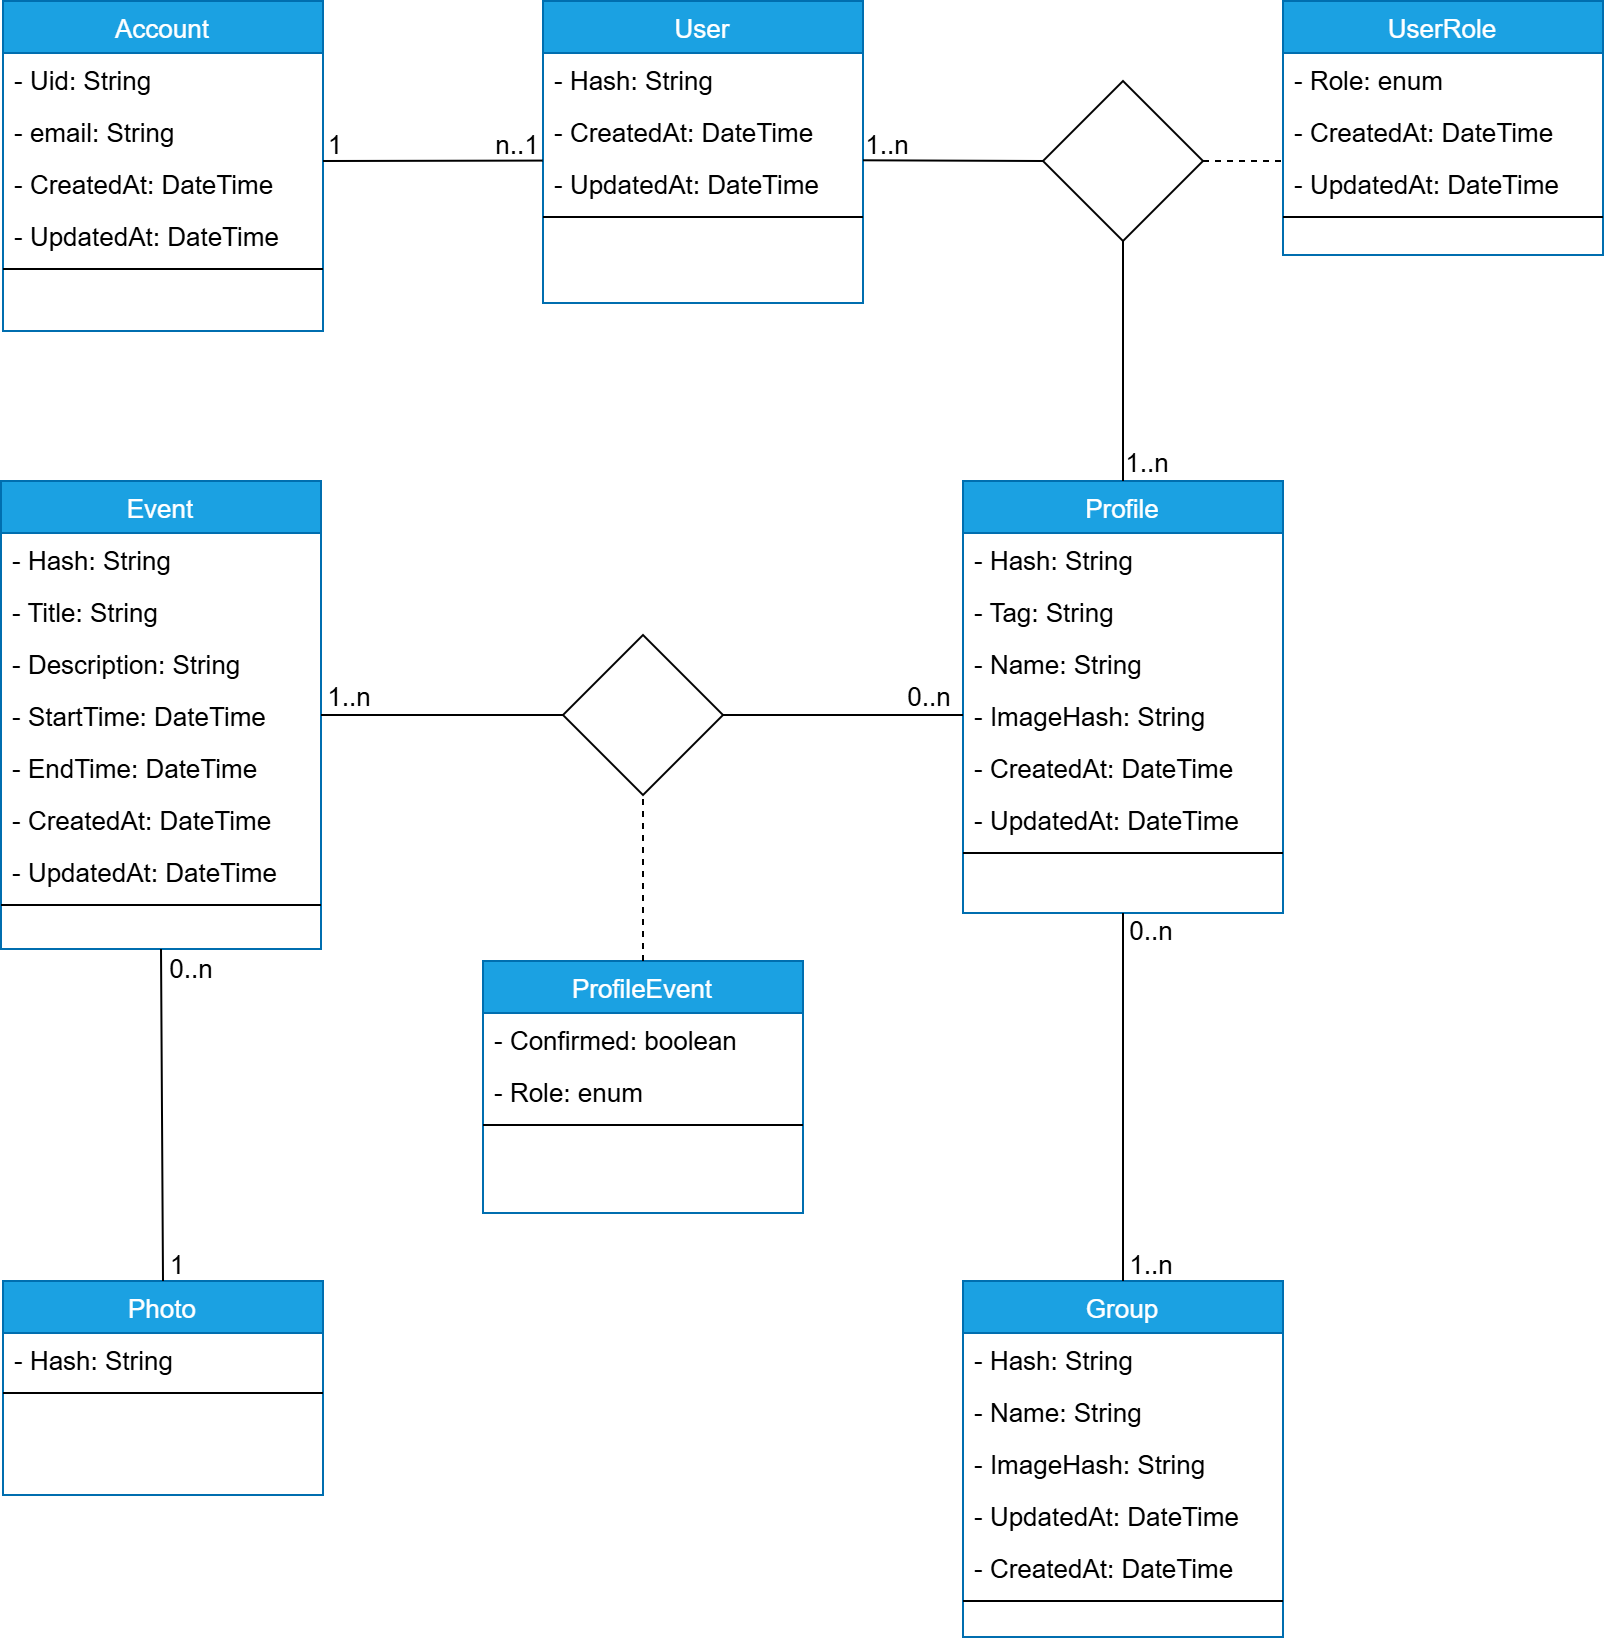
\includegraphics[width=\textwidth]{ProgettoDominioServer.png}
    \caption{Diagramma del dominio di Wyd}
\end{figure}

\clearpage
Le entità Account, User e Profile, assieme alla relazione UserRole,
descrivono le specifiche di autenticazione, identificazione dell'utente e i suoi ruoli sui profili associati.
I loro dati vengono recuperati solamente una volta nel ciclo di vita del programma,
a seguito del login dell'utente.
Vengono poi salvati in memoria locale,
riducendo il numero di richieste relative successive a un controllo su eventuali aggiornamenti.
Si prevede che le modifiche a questi elementi siano sporadiche.\\
Allo stesso modo gli oggetti Group vengono recuperati solo all'avvio dell'applicazione, e,
salvo rari aggiornamenti, non comportano ulteriori richieste.
Le richieste di lettura e scrittura previste per questi elementi sono quindi in quantità esigua,
e influiscono secondariamente sulle performance del sistema.\\
\\
La maggioranza delle richieste verterà sull'ottenimento dei dati relativi agli Event e ai Profile.
Gli Event descrivono gli impegni ai quali i profili partecipano.
Essendo la loro relazione di tipologia molti a molti,
si introduce l'entità ProfileEvent che descrive l'associazione evento-profilo,
indicando che un evento è condiviso con un profilo.
La proprietà più importante di ProfileEvent è sicuramente Confirmed,
una variabile booleana che esprime la partecipazione o meno di un profilo all'evento.
È ragionevole prevedere che la cardinalità dei profili associati a un evento non superi l'ordine delle centinaia.
Agli eventi che si associano ai profili l'ordine di grandezza invece previsto risiede nelle migliaia.
Ci sono molteplici situazioni da tenere in considerazione analizzando questa relazione.\\
\\
Sicuramente bisogna considerare il recupero specifico delle entità Event e Profile.
Questo accade quando un utente decide di entrare nel dettaglio di uno dei due elementi,
comportando la richiesta di tutti i dati dell'oggetto.
Consistono in un'operazione di lettura tutto sommato semplice:
essendo l'utente in possesso dell'identificativo dell'elemento,
la ricerca risulta diretta, e i dati da recuperare esigui.\\
\\
La conferma o la disdetta a un evento vede la modifica di un ProfileEvent.
Questa operazioni di per sé risulta veloce
in quanto necessita di recuperare un solo elemento per poi modificarlo.
Allo stesso modo la modifica di un evento comporta l'aggiornamento di un solo oggetto Event,
a seguito però del recupero del ProfileEvent associato,
necessario per controllare i permessi del profilo sull'evento.
Entrambe le operazioni richiedono però l'invio di una notifica verso tutti i profili interessati,
che necessita il recupero di tutti i ProfileEvent associati ogni volta che una di queste accade.\\
\\
La probabilità che un evento o un qualunque ProfileEvent a esso associato
venga modificato risulta quindi complessivamente elevata e, di conseguenza,
l'operazione di recupero degli identificativi di tutti i profili associati all'evento
è da considerarsi frequente.
Questa operazione, in base all'implementazione, può risultare costosa:
una separazione, un accoppiamento debole o la mancanza di indici tra Event e ProfileEvent
determinano la necessità di ricercare le entità in tutto il database.\\
\\
Quando un utente accede per la prima volta su un dispositivo
è necessario ottenere gli eventi associati ai suoi profili.
Allo stesso modo, a ogni avvio dell'applicazione si recuperano gli eventi
che hanno subito modifiche dall'ultimo accesso.
Inoltre, per poter garantire(all'interno di un determinato vincolo temporale)
la consistenza dei dati anche a livello locale,
il client applica una strategia di long polling
per ottenere gli eventi che sono stati modificati dall'ultimo aggiornamento noto.
L'operazione di ritrovamento degli eventi a partire dal profilo risulta quindi centrale e frequente,
per quanto possa accettare un tempo di esecuzione leggermente più lungo. \\

\begin{longtable}{|P{9.5cm}|P{2.5cm}|P{2.5cm}|}
    \hline
    \textbf{Funzionalità}                           & \textbf{Frequenza } & \textbf{Complessità} \\
    \hline
    Recupero di un Event                            & Media               & Semplice             \\
    \hline
    Recupero di un Profile                          & Media               & Semplice             \\
    \hline
    Modifica di un Event                            & Media               & Semplice             \\
    \hline
    Conferma/disdedda di un Event                   & Alta                & Semplice             \\
    \hline
    Ritrovamento dei Profile associati a un Event   & Alta                & Complessa            \\
    \hline
    Ritrovamento degli Event associati a un Profile & Alta                & Complessa            \\
    \hline
    \caption{Funzionalità principali tra Event e Profile}
\end{longtable}

La relazione tra Event e Photo impatta sulle prestazioni del sistema solo in casi particolari e
verrà affrontato nei capitoli successivi.
\clearpage